\chapter{Realization}\label{sec:realization}

The realization of the project can be separated into three distinct parts: \textbf{creating the wall model}, \textbf{creating hold models} and the \textbf{editor implementation}.
Each of the respective parts are open-source projects on GitHub, licensed under GPLv3:
\begin{itemize}
	\item \raisebox{-0.08em}{\includesvg[height=0.85 \baselineskip]{images/clis.svg}} -- the climber's scanner \cite{clis}
	\item \raisebox{-0.08em}{\includesvg[height=0.85 \baselineskip]{images/cled.svg}} -- the climber's editor \cite{cled}
\end{itemize}

Agisoft Metashape was used for 3D model generation.
While there are other suitable photogrammetry programs such as Meshroom (free), 3DF Zephyr (commercial) and COLMAP (free), Metashape was chosen for the following reasons:
\begin{itemize}
	\item It created the highest quality models out of the tested programs, given a representative sample\footnote{A foothold, a few regular holds and a dual texture hold, testing with 9, 12 and 15 images.} of the hold images.
	\item It includes a well-documented Python API, along with a good GUI.
\end{itemize}

Besides photogrammetry, another option that was considered for generating the models was laser scanning.
This was not a viable option because of the price, because products that could be used (such as Revopoint POP, XYZ 1.0 Pro or the Creality 3D Scanner) cost upwards of $400$\$ dollars, which is non-trivial considering only a potential quality improvement.

However, since a number of the aforementioned photogrammetry programs support laser scanning out of the box, the current approach could be combined with laser scanning in the future with only minor changes and a reasonable quality improvement, namely with more problematic holds (see section \ref{sec:dual}).

\section{Creating the wall model}
The wall model (figure \ref{fig:model}) has been created semi-automatically.

First, a set of 188 images was used by the Agisoft Metashape software to create a reference model.
This model was then manually edited in Blender 3D to remove modelling errors -- since the wall consists only of straight segments, this was done relatively easily.
After manual changes, the resulting model was reimported to Metashape to be textured.

\begin{figure}[t]
	\centering
	\includegraphics[width=\columnwidth]{images/wall/image.png}
	\caption{The model of the Smíchoff wall, created using Metashape and Blender.}
	\label{fig:model}
\end{figure}


\section{Creating hold models}
Since a regular climbing wall contains hundreds or even thousands of holds of varying sizes, it would be infeasible to model each of them manually.
It is important to automate as many steps as possible so that the amount of manual work done is minimized.

This has been accomplished using a turntable-based workflow, upon which the holds are placed and scanned.
The turntable turns the hold around for a stationary camera to take photos, which are then fed into the Agisoft Metashape protogrammetry software (+ Blender for post-processing).

The resulting workflow can model a single hold in 40 seconds of scanning (varying depending on the lighting conditions and the number of photos, the default being $12$) and additional $4$ minutes of processing.

\subsection{Turntable design}
A three stepper-motor turntable has been developed and 3D printed using the Fusion 360 CAD software and an Ender Pro 5 3D printer (figure \ref{fig:turntable}).
An Arduino board and A4988 motor controllers are used for fine motor control (figure \ref{fig:wiring}).
The communication with the Arduino is implemented via the serial port.

\begin{figure}
	\centering
	\includesvg[width=\columnwidth]{images/wiring.svg}
	\caption{The wiring diagram of the turntable, created using Fritzing.}
	\label{fig:wiring}
\end{figure}

To minimize the amount of friction, the only points of contact between the top and bottom part are 7 bearings (6 placed in a circular pattern and 1 placed in the middle).
Additionally, gears mounted to the motors turn the top of the turntable, achieving a $90/12 = 7.5$ reduction.
This allows the turntable to handle objects of weight up to \SI{8}{\kilo\gram}, with heavier objects requiring manual turning.

\begin{figure}
	% opravdu doufám, že tenhle kód nikdo číst nebude lmao
	\centering
	\subfloat[\centering Top part.]{{\includegraphics[height=3.6cm]{images/turntable/top.png} }}%
	\hfill
	\subfloat[\centering Base part (side).]{{\includegraphics[height=3.6cm]{images/turntable/side.png} }}%
	\hfill
	\subfloat[\centering Base part (top).]{{\includegraphics[height=3.6cm]{images/turntable/bottom.png} }}%
	\\
	\qquad
	\qquad
	\subfloat[\centering Motor mount.]{{\includegraphics[height=2.6cm]{images/turntable/mount.png} }}%
	\hfill
	\subfloat[\centering Motor gear (side).]{{\includegraphics[height=2.6cm]{images/turntable/gear-side.png} }}%
	\hfill
	\subfloat[\centering Motor gear (top).]{{\includegraphics[height=2.6cm]{images/turntable/gear-top.png} }}%
	\qquad
	\qquad
	\quad
	\qquad
	\caption{Parts of the model of the turntable, created using Fusion360.}%
	\label{fig:turntable}
\end{figure}

The top area is connected to a plexiglass with a marked center and 4 markers.

\subsection{Environment setup}
Two LED lights, mounted on adjustable stands and covered with baking paper (for light diffusion) were used to achieve good lighting conditions.
A large black cloth was used as the background to minimize the number of unwanted image features (see figure \ref{fig:setup}).

Additionally, since the camera is static, 300 ISO and 22 f/s were used to maximize the image quality.
This meant that the exposure time was usually around \SI{1.5}{\second}.
The f-stop was maximized to widen the focal plane, which puts the entire scanned object into focus and thus improves model quality.

The entire setup can be carried in a backpacking pack\footnote{Excluding the plexiglass, which is inflexible, and the camera, which is fragile.}, making it portable.
Additionally, all of the setup components (excluding the camera) can be purchased for under $4000$ CZK (or $180$ USD), making it affordable.

\begin{figure}
	\centering
	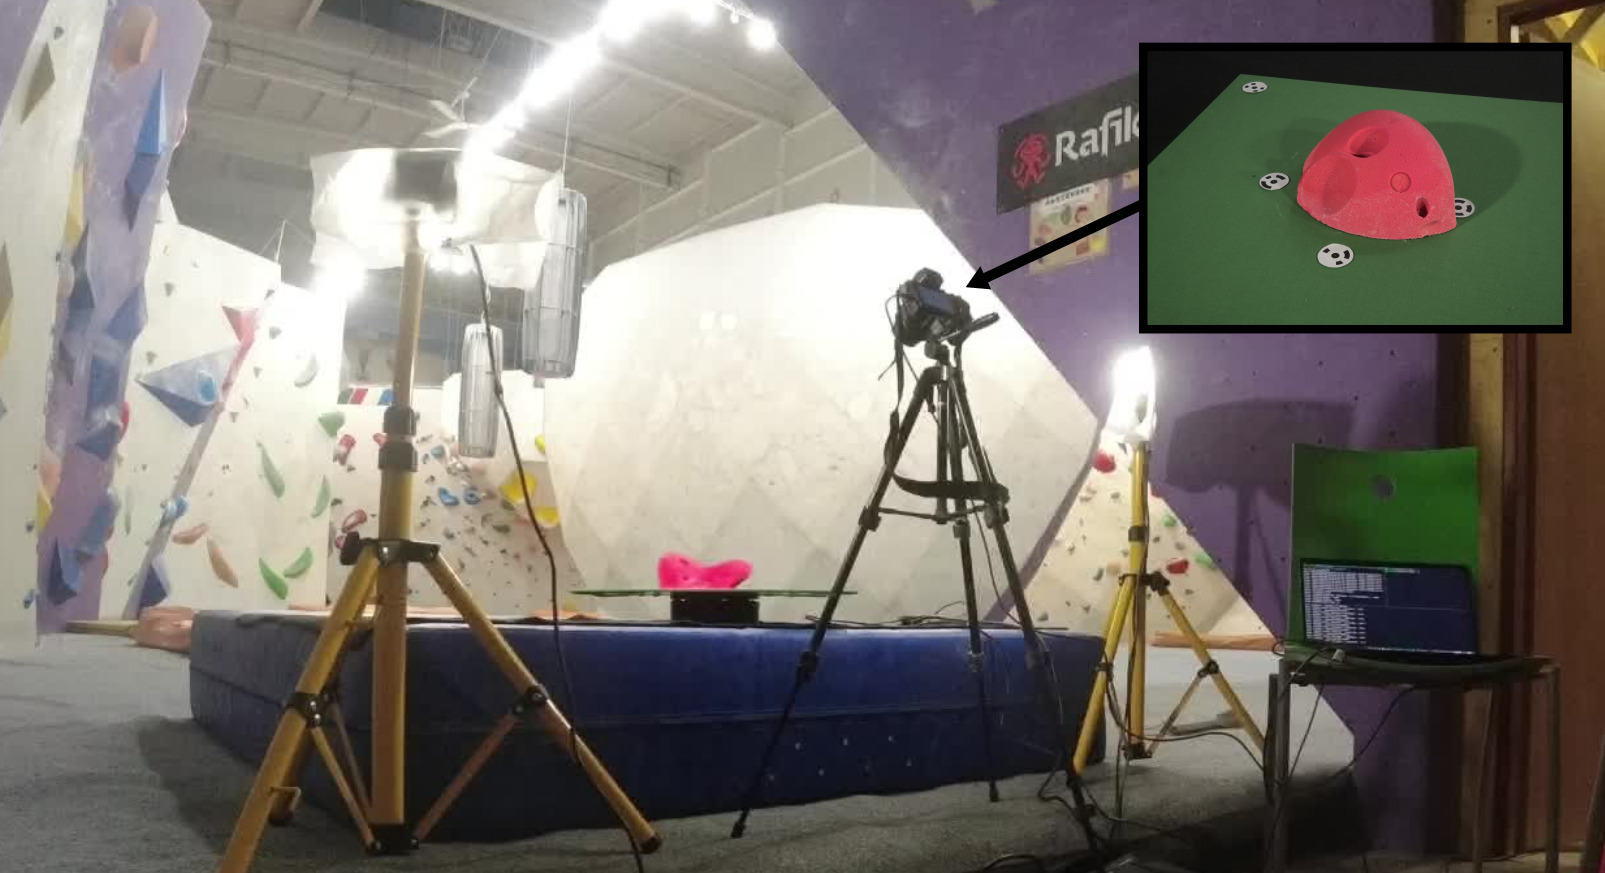
\includegraphics[width=\columnwidth]{images/setup/setup.png}
	\caption{An image of the setup during scanning, including the taken image. f-stop: 22, focal length: \SI{38}{\milli\meter}, ISO: 320, exposure time: \SI{1}{\second}.}
	  
	\label{fig:setup}
\end{figure}

\subsection{Image masking}
The photogrammetry software expects the images to be viewed from various angles, as outlined in section \ref{sec:theory}.
This poses a problem for the turntable setup, since the background might not be perfectly dark and thus create undesired feature points that make it harder to reconstruct the model.
Fortunately, the contrast between the top of the turntable and the background is large enough to automatically construct a mask to filter the background out.
This is done using the OpenCV library (as seen in figure \ref{fig:mask}) by
\begin{enumerate}
	\item converting the image to grayscale,
	\item generating a binary image using a threshold on the pixel brightness,
	\item applying a contour-generating algorithm \cite{suzuki1985topological} on the image and finally
	\item using the largest (flood-filled) contour as the image mask.
\end{enumerate}

\begin{figure}
	% opravdu doufám, že tenhle kód nikdo číst nebude lmao
	\centering
	\subfloat[\centering Original photo.]{{\includegraphics[height=2.0cm]{images/masking/hold.png} }}%
	\hfill
	\subfloat[\centering Hold contours.]{{\includegraphics[height=2.0cm]{images/masking/contourimage.jpg} }}%
	\hfill
	\subfloat[\centering Generated mask.]{{\includegraphics[height=2.0cm]{images/masking/mask.jpg} }}%
	\hfill
	\subfloat[\centering Resulting photo.]{{\includegraphics[height=2.0cm]{images/masking/resulting.jpg} }}%
	\caption{The process of masking a hold, generated using OpenCV.}%
	\label{fig:mask}
\end{figure}

\subsection{Dual texture holds}\label{sec:dual}
Glossy surfaces are a problematic type of surfaces for photogrammetry, since the angle under which they are viewed changes their appearance due to light reflections.
This problem is realized in „dual-texture“ holds which, as the name suggests, contain two textures -- a mate texture that is meant for the climber to hold (or step) onto, and the glossy texture which is usually not.

A standard way of dealing with glossy surfaces is to cover them in something that is mate.
While this does solve the problem of model generation, it ruins the texture, because the mate solution is usually opaque, thus requiring another set of images for texturing.

In our case, however, the solution is pretty straightforward -- cover them in climbing chalk (figure \ref{fig:chalk}).
Since it is mate, it reduces the reflections of the glossy surface and provides additional feature points, making it easier for the photogrammetry software to reconstruct the model.
Additionally, since climbing chalk will be applied to the holds by climber during regular usage anyway, there is no need to obtain more images for texturing.

It is worth noting that this solution is not perfect -- since the chalk doesn't cover the hold entirely, some reflections persist and can introduce model inaccuracies.
In such cases, manual modelling using Blender to reconstruct the missing hold parts is required.

\begin{figure}[h]
	\centering
	\subfloat{{\includegraphics[height=2.5cm]{images/holds/1.png} }}%
	\hfill
	\subfloat{{\includegraphics[height=2.5cm]{images/holds/4.png} }}%
	\hfill
	\subfloat{{\includegraphics[height=2.5cm]{images/holds/3.png} }}%
	\caption{Example of holds with chalk applied. Some reflections are still visible, but they are not as pronounced as with no chalk applied.}%
	\label{fig:chalk}
\end{figure}

\subsection{Hold metadata}
After all models have been generated, a \verb|yaml| metadata file is created for storing their properties.
It is a dictionary, with keys being the hold models and the attributes their properties.
The specification of a single item is as follows:

\begin{minted}{yaml}
<the first 12 characters of the sha256sum of model data>:
  color: [<name>, <hex value>]                 # strings
  type: <the type of hold>                     # string
  manufacturer: <the name of the manufacturer> # string
  labels: [<list>, <of>, <custom>, <labels>]   # strings
  volume: <a float volume of the hold>         # float
  date: <the date the hold model was created>  # datetime
\end{minted}

All of the specified attributes are optional.
Some of them (like volume and date) are automatically inferred, while others have to be added manually.
The first 12 characters of the hashsum were chosen for readability purposes and because millions of holds would be required for a reasonable chance of collision\footnote{Since there are 16 symbols, the total pool of hashes is $N = 16^{12}$. We'll take $n = 10\ 000$ as the maximum number of holds. The chance of collision is inverse to there not being one in the first $n$ holds, which can be calculated as $1 - \prod_{i = 1}^{n} \frac{N - i}{N} \approx 1.77 \cdot 10^{-7}$, which is more than reasonable.}.

\section{Editor implementation}
The editor has been created using the Unity editor, with the majority of the codebase being written in C\#.
While other options exist, such as Unreal Engine and Godot, Unity was chosen due to the author's experience with developing games using it, along with a large ecosystem of packages that could be used to simplify the implementation and allow for rapid prototyping.

Using this ecosystem, a number of freely available packages were used (with minor code modifications), namely

\begin{itemize}
	\item \textbf{Quick Outline} \cite{quickoutline} -- object outline creator,
	\item \textbf{Runtime OBJ Importer} \cite{objimport} -- an \verb|.obj| file importer and
	\item \textbf{Unity Standalone File Browser} \cite{unitystandalonefilebrowser} -- a cross-platform file browser.
\end{itemize}

The editor code is open-source and cross-platform (Mac, Windows, Linux), with newest releases (along with their changelog) being freely available at the \href{https://github.com/Climber-Tools/Cled/releases}{project releases page}.
Each release is automatically built from the source code using GitHub Actions on tagged commits.
The version numbering scheme follows Semantic Versioning 2.0.

\subsection{Movement}
Movement is implemented using keyboard in a way commonly used in 3D programs.
The arrow or \verb|WSAD| keys provide left, right, forward and backward movement, while the \verb|Space| and \verb|Shift| keys allow flying up and down.

Physics and gravity are also implemented, with the character being pulled to the ground when not flying, and colliding with both the wall and the holds.

\subsection{Wall and hold format}
For the editor to correctly load the scene, it expects the wall and holds to be in the \verb|obj| file format, possibly with a \verb|mtl| file and a bitmap texture.
It has specific requirements on naming and location of the files which differs slightly from Clis.
This is because the editor uses only a subset of the files generated from Clis along with a few that Clis doesn't generate.
To make things easier, the editor contains a Python script to automatically import models from Clis and generate the missing files, which are preview images and preview videos.

The wall can also contain a \verb|yaml| metadata file for wall-specific things, namely the route grades, the names of the setters and which zone the route is located in.
This is to simplify editing route properties by selecting the right option from a dropdown, instead of having to manually type it in.
Here is an example of one such file:

\begin{minted}{yaml}
Grades: ["black", "purple", "red", "salmon", "blue", "yellow"]
Setters: ["Danny", "Bert"]
Zones: ["1", "2", "3", "4", "5"]
\end{minted}

\subsection{Editor modes}
The editor contains three modes in which can operate, with the current mode being always displayed in the top right.
While this might seem like an implementation detail, it is important for user documentation and general usage, because the user always knows which state the editor is in.
An obvious inspiration is the Vim text editor, which makes the mode distinction similarly apparent.

The modes are the following:

\begin{itemize}
	\item \textbf{NORMAL} -- the mode the user is normally in; hovering highlights holds, which can be either picked up or selected.
	\item \textbf{HOLDING} -- the mode in which the user is holding a specific hold and can place it, or switch to the next one from the selection.
	\item \textbf{ROUTE} -- the mode in which the user is modifying the selected route by adding/removing new holds, or modifying route parameters.
\end{itemize}

\subsection{Hold selection}
Quickly selecting which holds to place on the wall is crucial for effective virtual route setting, because it dictates the time the route setting takes.
The editor contains a menu (accessed via pressing either \verb|Tab| or \verb|Q|) from which a subset of holds can be filtered and cycled while editing.

Filtering holds can be done by selecting a specific hold color, type, manufacturer, or custom hold label.
By default, the currently filtered holds are also sorted first by their color, then by their type, and finally by their volume.
Additionally, hovering on each of the menu items rotates them around, which is useful when the static hold image isn't descriptive enough.

\subsection{Import and Export}
The import and export format for the project files is a human-readable \verb|yaml| file containing information about the state of the holds, routes, paths to the models and other metadata.
This makes it easy to be used in other applications (both for viewing and modification), since it is well readable and parseable.
Here is how the format looks like:

\begin{minted}{yaml}
Version: 2.1.0 # Editor version (for compatibility reasons)

Player: # player settings
  Light: false # whether the player's light is on
  Position: # the player position as a vector
    x: 4.66010237
    y: 1.93126345
    z: -8.63198185
  Orientation: # the player orientation (up/down, left/right)
    x: 35.8053398
    y: 123.996086
  Flying: false # whether the player is currently flying

WallModelPath: /home/tom/Wall/wall.obj
HoldModelsPath: /home/tom/Holds

Holds: # a dictionary of hold instances
  f21cde933ad9: # a unique ID for the hold instance
    BlueprintId: 4bdff2704462 # an ID of the hold model
    State:
      Position: # the position of the hold in space
        x: 1.20504105
        y: 0.378549755
        z: -7.67928696
      Normal: # the normal of the hold, away from the wall
        x: 0.994500279
        y: 0.0156783238
        z: 0.103554823
      Rotation: 0 # the hold rotation about the normal
      Flipped: false # whether the hold is horizontally flipped
  0436ff53a1d8:
    BlueprintId: 4bdff2704462
    State:
      Position:
        x: 1.46525836
        y: 0.472094655
        z: -8.19389153
      Normal:
        x: 0.752805889
        y: -0.0226488542
        z: 0.657852829
      Rotation: 1.21387374
      Flipped: false

Routes: # a list of routes
- Name: A very nice route
  Grade: blue
  Zone: 3
  Setter: Danny
  HoldIDs: # which hold instances the route contains
  - 0436ff53a1d8
  - f21cde933ad9

StartingHoldIDs: # a list of starting holds
- f21cde933ad9

EndingHoldIDs: # a list of ending holds
- 0436ff53a1d8

SelectedHoldBlueprintIDs: # a list of currently selected holds
- f21cde933ad9
- 0436ff53a1d8

Lights: # a list of point lights around the wall
  Positions:
  - x: 3.71035504
    y: 3.53241396
    z: -7.11679459
  - x: 5.59678602
    y: 3.53241396
    z: -3.97351503
  Intensity: 0.2 # how strong they are
  ShadowStrength: 0.2 # how hard their shadows are

CaptureSettings: # image capture settings
  ImagePath: /home/tom/Pictures # captured images path
  ImageSupersize: 2 # captured images resolution scaling
\end{minted}

\subsection{Capturing images}
The editor contains functionality for capturing the current image of the wall.
This can be done anywhere in the editor by either selecting the option from the toolbar, or by pressing \verb|Ctrl+P| (see figure \ref{fig:capture} for examples).
The image is then saved to the default system „Pictures“ folder, unless configured otherwise in the settings.

\begin{figure}[h]
	\centering
	\subfloat{{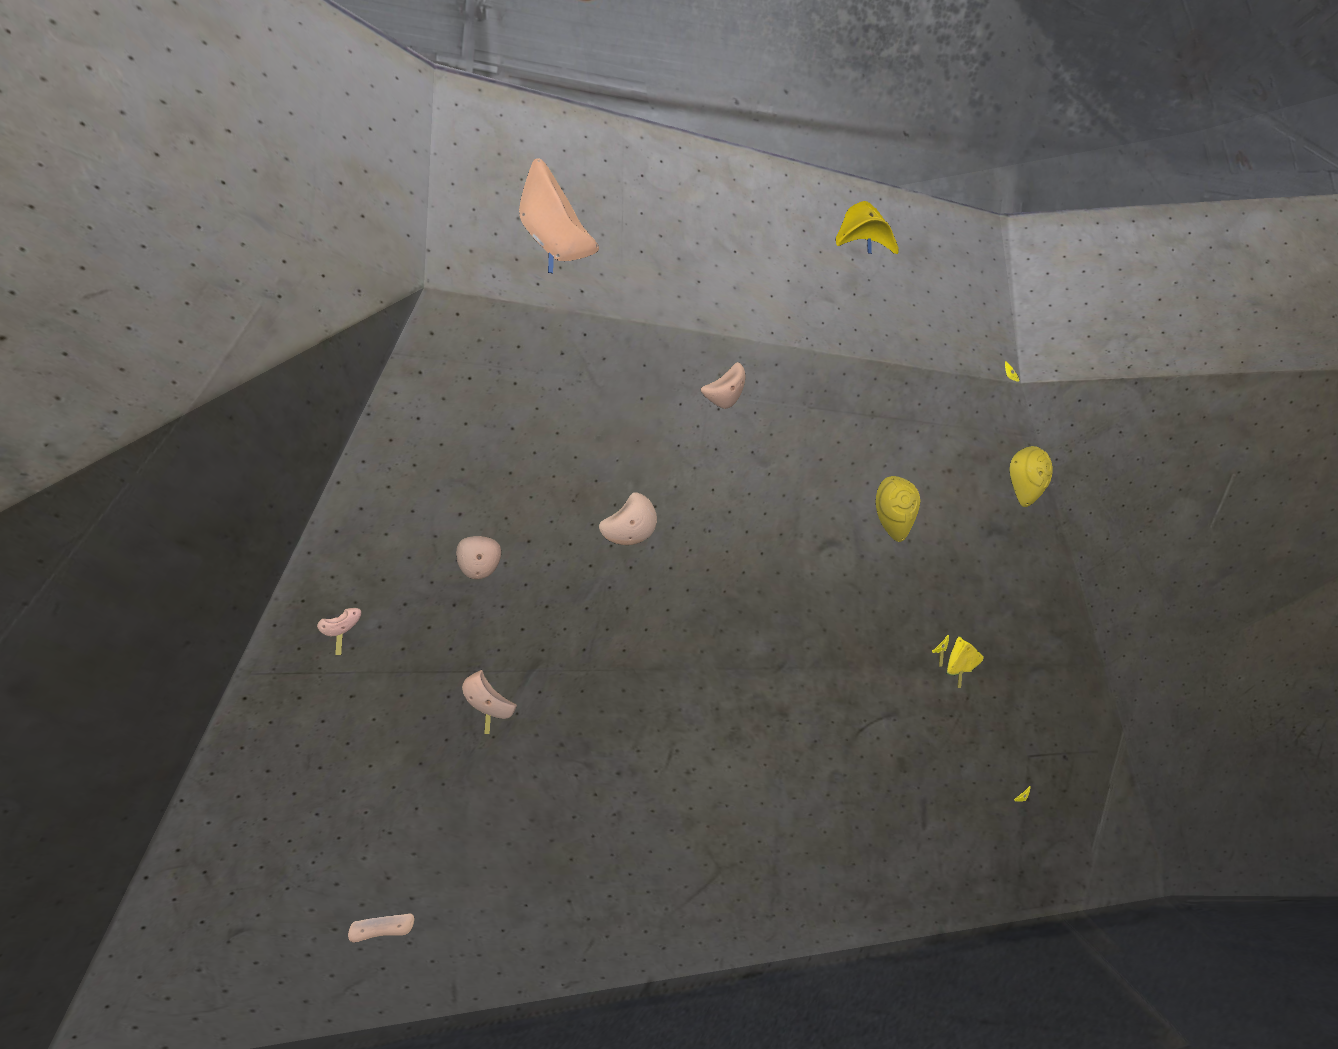
\includegraphics[height=5cm]{images/editor/capture-1.png} }}%
	\hfill
	\subfloat{{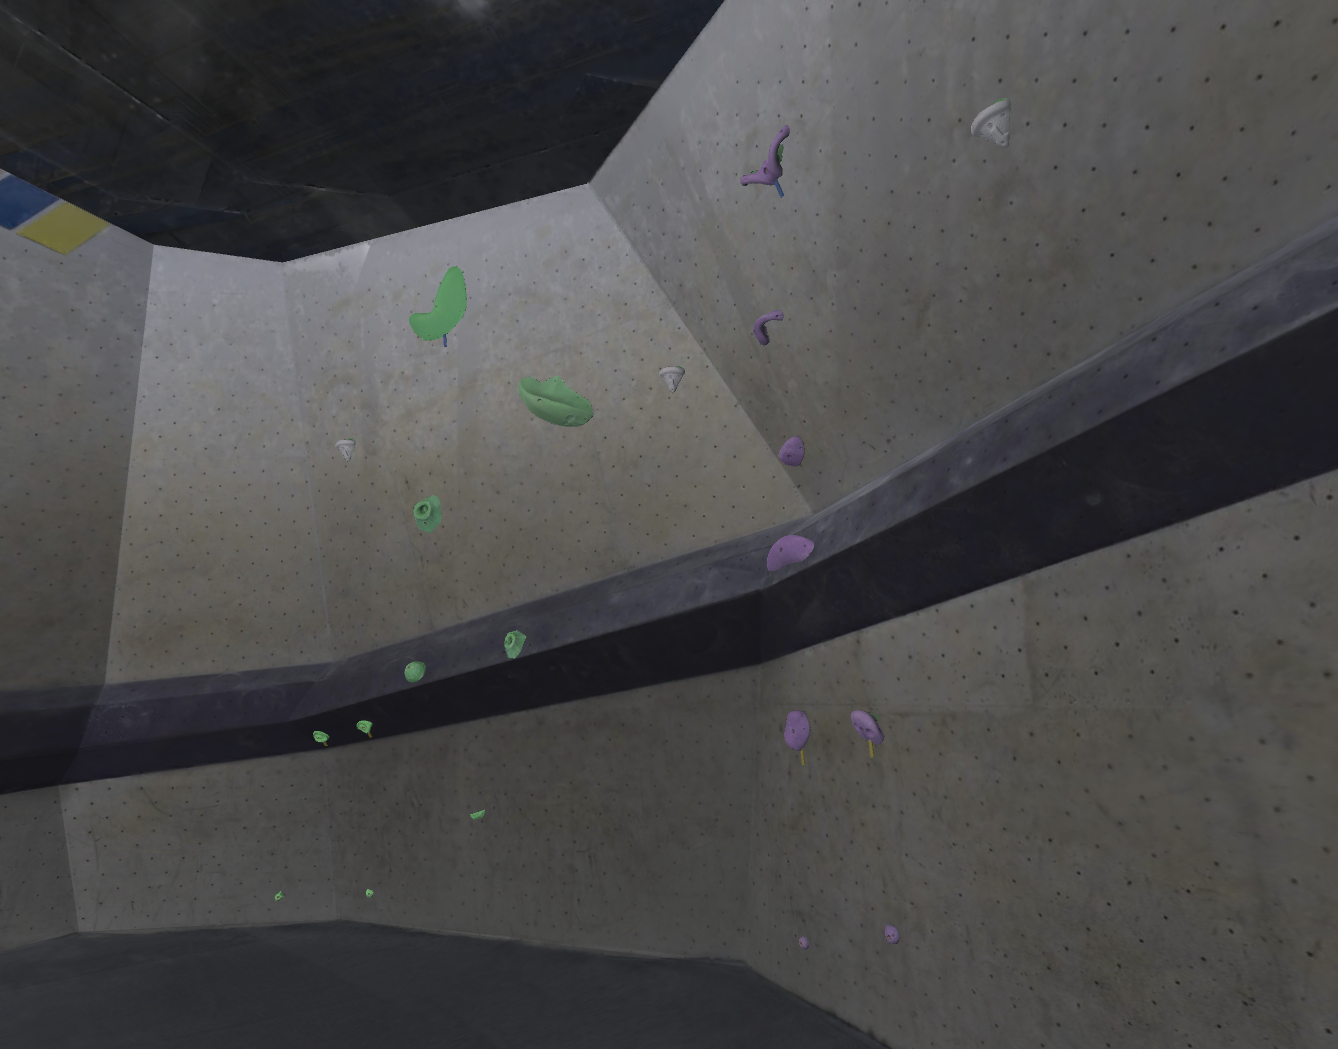
\includegraphics[height=5cm]{images/editor/capture-2.png} }}%
	\caption{Images generated using the editor capture functionality.}%
	\label{fig:capture}
\end{figure}

\subsection{Lighting}
Since each wall has different lighting needs and specifying them in the wall metadata would be too impractical, the editor supports placing lights on the current player position (and removing them).
This can be done either from the \verb|Lighting| section of the toolbar, or by using \verb|F| to toggle the player lighting and \verb|Ctrl+F| to place one at the player position.

\subsection{Routesetter feedback}
To test the editor implementation functionality, two of Smíchoff's routesetters were asked to provide feedback regarding the editor usage.
The task was to construct the routes that they had built on the wall using the editor and an image for reference.
A number of useful recommendations were implemented based on this feedback, such as (TODO: potkávám se s nimi ve čtvrtek).
